\chapter{Prime numbers}
\epigraph[author={Mark Haddon},source={The Curious Incident of the Dog in the Night-Time}]{I think prime numbers are like life. They are very logical but you could never work out the rules, even if you spent all your time thinking about them.}\SubIndex{Haddon, Mark}

\section{Prime numbers}
A positive integer \(p \ge 2\) is \emph{prime}\define{prime} if the only positive integers which divide \(p\) are \(1\) and \(p\).

\begin{problem}{integers:two.prime}
Prove that \(2\) is prime and that \(3\) is prime and that \(4\) is not prime.
\end{problem}

\begin{lemma}
If \(b,c,d\) are integers and \(d\) divides \(bc\) and \(d\) is coprime to \(b\) then \(d\) divides \(c\).
\end{lemma}
\begin{proof}
Since \(d\) divides the product \(bc\), we can write the product as \(bc=qd\).
Since \(d\) and \(b\) are coprime, their greatest common divisor is \(1\).
So there are B\'ezout coefficients \(s,t\) for \(b,d\), so \(sb+td=1\).
So then \(sbc+tdc=c\), i.e. \(sqd+tdc=c\), or \(d(sq+dc)=c\), i.e. \(d\) divides \(c\).
\end{proof}

\begin{corollary}
A prime number divides a product \(bc\) just when it divides one of the factors \(b\) or \(c\).
\end{corollary}

An expression of a positive integer as a product of primes, such as \(12=2 \cdot 2 \cdot 3\), written down in increasing order, is a \emph{prime factorization}.
\marginpar
{\small
\begin{align*}
2 &= 2, \\
3 &= 3, \\
4 &= 2 \cdot 2, \\
5 &= 5, \\
6 &= 2 \cdot 3, \\
7 &= 7, \\
8 &= 2 \cdot 2 \cdot 2, \\
9 &= 3 \cdot 3, \\
10 &= 2 \cdot 5, \\
11 &= 11, \\
12 &= 2 \cdot 2 \cdot 3, \\
&\ \vdots \\
2395800 &= 2^3 \cdot 3^2 \cdot 5^2 \cdot 11^3, \\
&\ \vdots
\end{align*}
}
\begin{theorem}
Every positive integer \(n\) has a unique prime factorization.
\end{theorem}
\begin{proof}
\emph{Danger:} if we multiply together a collection of integers, we must insist that there can only be finitely many numbers in the collection, to make sense out of the multiplication.

\emph{More danger:} an \emph{empty} collection is always allowed in mathematics.
We will simply say that if we have \emph{no} numbers at all, then the product of those numbers (the product of no numbers at all) is defined to mean \(1\).
This will be the right definition to use to make our theorems have the simplest expression.
In particular, the integer \(1\) has the prime factorization consist of \emph{no} primes.

First, let's show that there is a prime factorization, and then we will see that it is unique.
It is clear that \(1, 2, 3, \dots, 12\) have prime factorizations, as in our table above.
Suppose that all integers \(1,2,\dots,n-1\) have prime factorizations.
If \(n\) does not factor into smaller factors, then \(n\) is prime and \(n=n\) is a factorization.
Suppose that \(n\) factors, say into a product \(n=bc\) of positive integers, neither equal to \(1\).
Write down a prime factorization for \(b\) and then next to it one for \(c\), giving a prime factorization for \(n=bc\).
So every positive integer has at least one prime factorization.

Let \(p\) be the smallest integer so that \(p \ge 2\) and \(p\) divides \(n\).
Clearly \(p\) is prime.
Since \(p\) divides the product of the primes in any prime factorization of \(n\), so \(p\) must divide one of the primes in the factorization.
But then \(p\) must equal one of these primes, and must be the smallest prime in the factorization.
This determines the first prime in the factorization. 
So write \(n=pn_1\) for a unique integer \(n_1\), and by induction we can assume that \(n_1\) has a unique prime factorization, and so \(n\) does as well.
\end{proof}

\begin{theorem}[Euclid]\SubIndex{Euclid}
There are infinitely many prime numbers.
\end{theorem}
\begin{proof}
Write down a list of finitely many primes, say \(p_1, p_2, \dots, p_n\).
Let \(b\defeq p_1 p_2 \dots p_n\) and let \(c\defeq b+1\).
Then clearly \(b,c\) are coprime.
So the prime decomposition of \(c\) has none of the primes \(p_1, p_2, \dots, p_n\) in it, and so must have some other primes distinct from these.
\end{proof}

\begin{problem}{primes:Eratosthenes}
Write down the positive integers in a long list starting at \(2\):
\[
2, 3, 4, 5, 6, 7, 8, 9, 10, 11, 12, 13, 14, 15, 16, \dots
\]
Strike out all multiples of \(2\), except \(2\) itself:
\[
2, 3, {\color{gray}4}, 5, {\color{gray}6}, 7, {\color{gray}8}, 9, {\color{gray}10}, 11, {\color{gray}12}, 13, {\color{gray}14}, 15, {\color{gray}16}, \dots
\]
Skip on to the next number which isn't struck out: \(3\).
Strike out all multiples of \(3\), except \(3\) itself:
\[
2, 3, {\color{gray}4}, 5, {\color{gray}6}, 7, {\color{gray}8}, {\color{gray}9}, {\color{gray}10}, 11, {\color{gray}12}, 13, {\color{gray}14}, {\color{gray}15}, {\color{gray}16}, \dots
\]
Skip on to the next number which isn't struck out, and strike out all of its multiples except the number itself.
Continue in this way forever.
Prove that the remaining numbers, those which do \emph{not} get struck out, are precisely the prime numbers.
Use this to write down all prime numbers less than \(120\).
\end{problem}
\begin{answer}{primes:Eratosthenes}
2, 3, 5, 7, 11, 13, 17, 19, 23, 29, 31, 37, 41, 43, 47, 53, 59, 61, 67, 71, 73, 79, 83, 89, 97, 101, 103, 107, 109, 113
\end{answer}

\section{Greatest common divisors}

We speed up calculation of the greatest common divisor by factoring out any obvious common factors: \(\gcd{46,12}=\gcd{2 \cdot 23,2 \cdot 6}=2 \gcd{23,6}=2\).
For example, this works well if both numbers are even, or both are multiples of ten, or both are multiples of 5, or even if both are multiples of 3.

\begin{problem}{integer:multiples.of.three}
Prove that an integer is a multiple of 3 just when its digits sum up to a multiple of 3.
Use this to see if \(12345\) is a multiple of \(3\).
Use this to find \(\gcd{12345,123456}\).
\end{problem}

\begin{problem}{integers:multiple.of.two}
An \emph{even integer}\define{even integer} is a multiple of \(2\); an \emph{odd integer}\define{odd integer} is \emph{not} a multiple of \(2\).
Prove that if \(b,c\) are positive integers and 
\begin{enumerate}
\item
\(b\) and \(c\) are both even then \(\gcd{b,c}=2\gcd{b/2,c/2}\),
\item
\(b\) is even and \(c\) is odd, then \(\gcd{b,c}=\gcd{b/2,c}\),
\item
\(b\) is odd and \(c\) is even, then \(\gcd{b,c}=\gcd{b,c/2}\),
\item
\(b\) and \(c\) are both odd, then \(\gcd{b,c}=\gcd{b,b-c}\).
\end{enumerate}
Use this to find the greatest common divisor of \(4864, 3458\) without using long division. Answer: \(\gcd{4864,3458}=19\).
\end{problem}
%\begin{sagesilent}
%def formatmultiplier(a):
%    if a==1:
%        return ""
%    else:
%        if a<0:
%            return "(-{})".format(-a)
%        else:
%            return "{}".format(a)
%    
%def bgcd(b,c,start=1):
%    result=formatmultiplier(start)+r"gcd\{" + "{},{}".format(b,c)+r"\}="
%    if b<0:
%        return result+bgcd(-b,c,start)
%    if c<0:
%        return result+bgcd(b,-c,start)
%    if b==1:
%        return result+"{}".format(start)
%    if c==1:
%        return result+"{}".format(start)
%    if b==0:
%        return result+"{}".format(start*c)
%    if c==0:
%        return result+"{}".format(start*b)
%    if is_even(b):
%        if is_even(c):
%            return result+bgcd(b/2,c/2,2*start)
%        else:
%            return result+bgcd(b/2,c,start)
%    else:
%        if is_even(c):
%            return result+bgcd(b,c/2,start)
%        else:
%            if b>c:
%                return result+bgcd(b-c,c,start)
%            else:
%                return result+bgcd(b,c-b,start)
%\end{sagesilent}
\begin{answer}{integers:multiple.of.two}
%\sagestr{bgcd(4864,3458)}
\begin{align*}
\gcd{4864,3458}&=2\gcd{2432,1729},\\&=2\gcd{1216,1729},\\&=2\gcd{608,1729},\\&=2\gcd{304,1729},\\&=2\gcd{152,1729},\\&=2\gcd{76,1729},\\&=2\gcd{38,1729},\\&=2\gcd{19,1729},\\&=2\gcd{19,1710},\\&=2\gcd{19,855},\\&=2\gcd{19,836},\\&=2\gcd{19,418},\\&=2\gcd{19,209},\\&=2\gcd{19,190},\\&=2\gcd{19,95},\\&=2\gcd{19,76},\\&=2\gcd{19,38},\\&=2\gcd{19,19},\\&=2\gcd{19,0},\\&=38\end{align*}
\end{answer}



\section{Sage}

\epigraph[author={Leonhard Euler}]{Mathematicians have tried in vain to this day to discover some order in the sequence of prime numbers, and we have reason to believe that it is a mystery into which the human mind will never penetrate.}\SubIndex{Euler, Leonhard}

Sage can factor numbers into primes: \verb!factor(1386)! gives \(2 \cdot 3^2 \cdot 7 \cdot 11\).
Sage can find the next prime number larger than a given number: \verb!next_prime(2005)!\(=\sage{next_prime(2005)}\).
You can test if the number \(4\) is prime with \verb!is_prime(4)!, which returns \verb!False!.
To list the primes between \(14\) and \(100\), type  \verb!prime_range(14,100)! to see
\begin{verbatim} 
[17, 19, 23, 29, 31, 37, 41, 43, 47, 53, 59, 61, 67, 71, 73, 79, 83, 89,
97]
\end{verbatim}
The number of primes less than or equal to a real number \(x\) is traditionally denoted \(\pi(x)\) (which has nothing to do with the \(\pi\) of trigonometry).
In sage, \(\pi(x)\) is denoted \verb!prime_pi(x)!.
For example, \(\pi(10^6)=\sage{prime_pi(10^6)}\) is calculated as \verb!prime_pi(10^6)!.
The prime number theorem says that \(\pi(x)\) gets more closely approximated by
\[
\frac{x}{-1+\log x}
\]
as \(x\) gets large.
We can plot \(\pi(x)\), and compare it to that approximation.
\begin{sageblock}
p=plot(prime_pi, 0, 10000, rgbcolor='red')
q=plot(x/(-1+log(x)), 5, 10000, rgbcolor='blue')
show(p+q)
\end{sageblock}
which displays:
\begin{center}
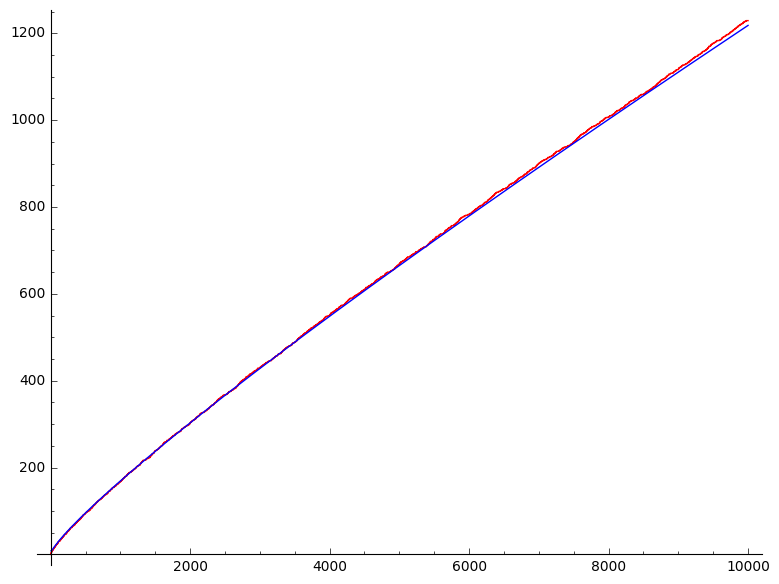
\includegraphics[width=10cm]{prime-pi}
\end{center}

\begin{problem}{integers:code}
Write code in sage to find the greatest common divisor of two integers, using the ideas of problem~\vref{problem:integers:multiple.of.two}.
\end{problem}
%def is_even(b):
%    return b%2==0
%
%def gcd_binary(b,c):
%    if b==0:
%        return c
%    else:
%        if c==0:
%            return b
%        else:
%            if is_even(b):
%                if is_even(c):
%                    return 2*gcd_binary(b//2,c//2)
%                else:
%                    return gcd_binary(b//2,c)
%            else:
%                if is_even(c):
%                    return gcd_binary(b,c//2)
%                else:
%                    B=abs(b)
%                    C=abs(c)
%                    if B>C:
%                        return gcd_binary(B,B-C)
%                    else:
%                        return gcd_binary(C,C-B)
